\section{Introduction}
The K-means clustering algorithm started to be developed in the middle of 20th century. The objective was seperating data into groups. Stuart Lloyd was the first to develop this algorithm in 1957 in Bell Labs, but his works were published until 1982. Around the same time, another researcher named Edward W. Forgy published a method in 1965 that was quite similar to Lloyd's work. Since both of the researcher have contributed to the method, algorithm is sometimes referred to by both their names as the Lloyd-Forgy algorithm. The found algorithm was so simple and effective, these features makes the algorithm extremely popular in various fields such as market segmentation where companies identify specific groups within their market to target them more effectively, and in image compression, which helps in reducing the size of image files without losing significant quality.

K-means clustering is a straightforward and widely used technique that organizes a dataset into K distinct groups. The primary aim is to allocate the data into clusters where the items within each cluster are as similar as possible, and items in different clusters are distinct from each other. This is achieved by minimizing the total distance between the data points and the centroid or the center point of the cluster they are assigned to. This method helps in creating clear distinctions between different groups, making it easier for businesses or analysts to derive insights from large sets of data.

\empty

Following example demonstrates the K-means clustering algorithm in a randomly generated 2D dataset. \\

\begin{figure}[H]
    \centering
    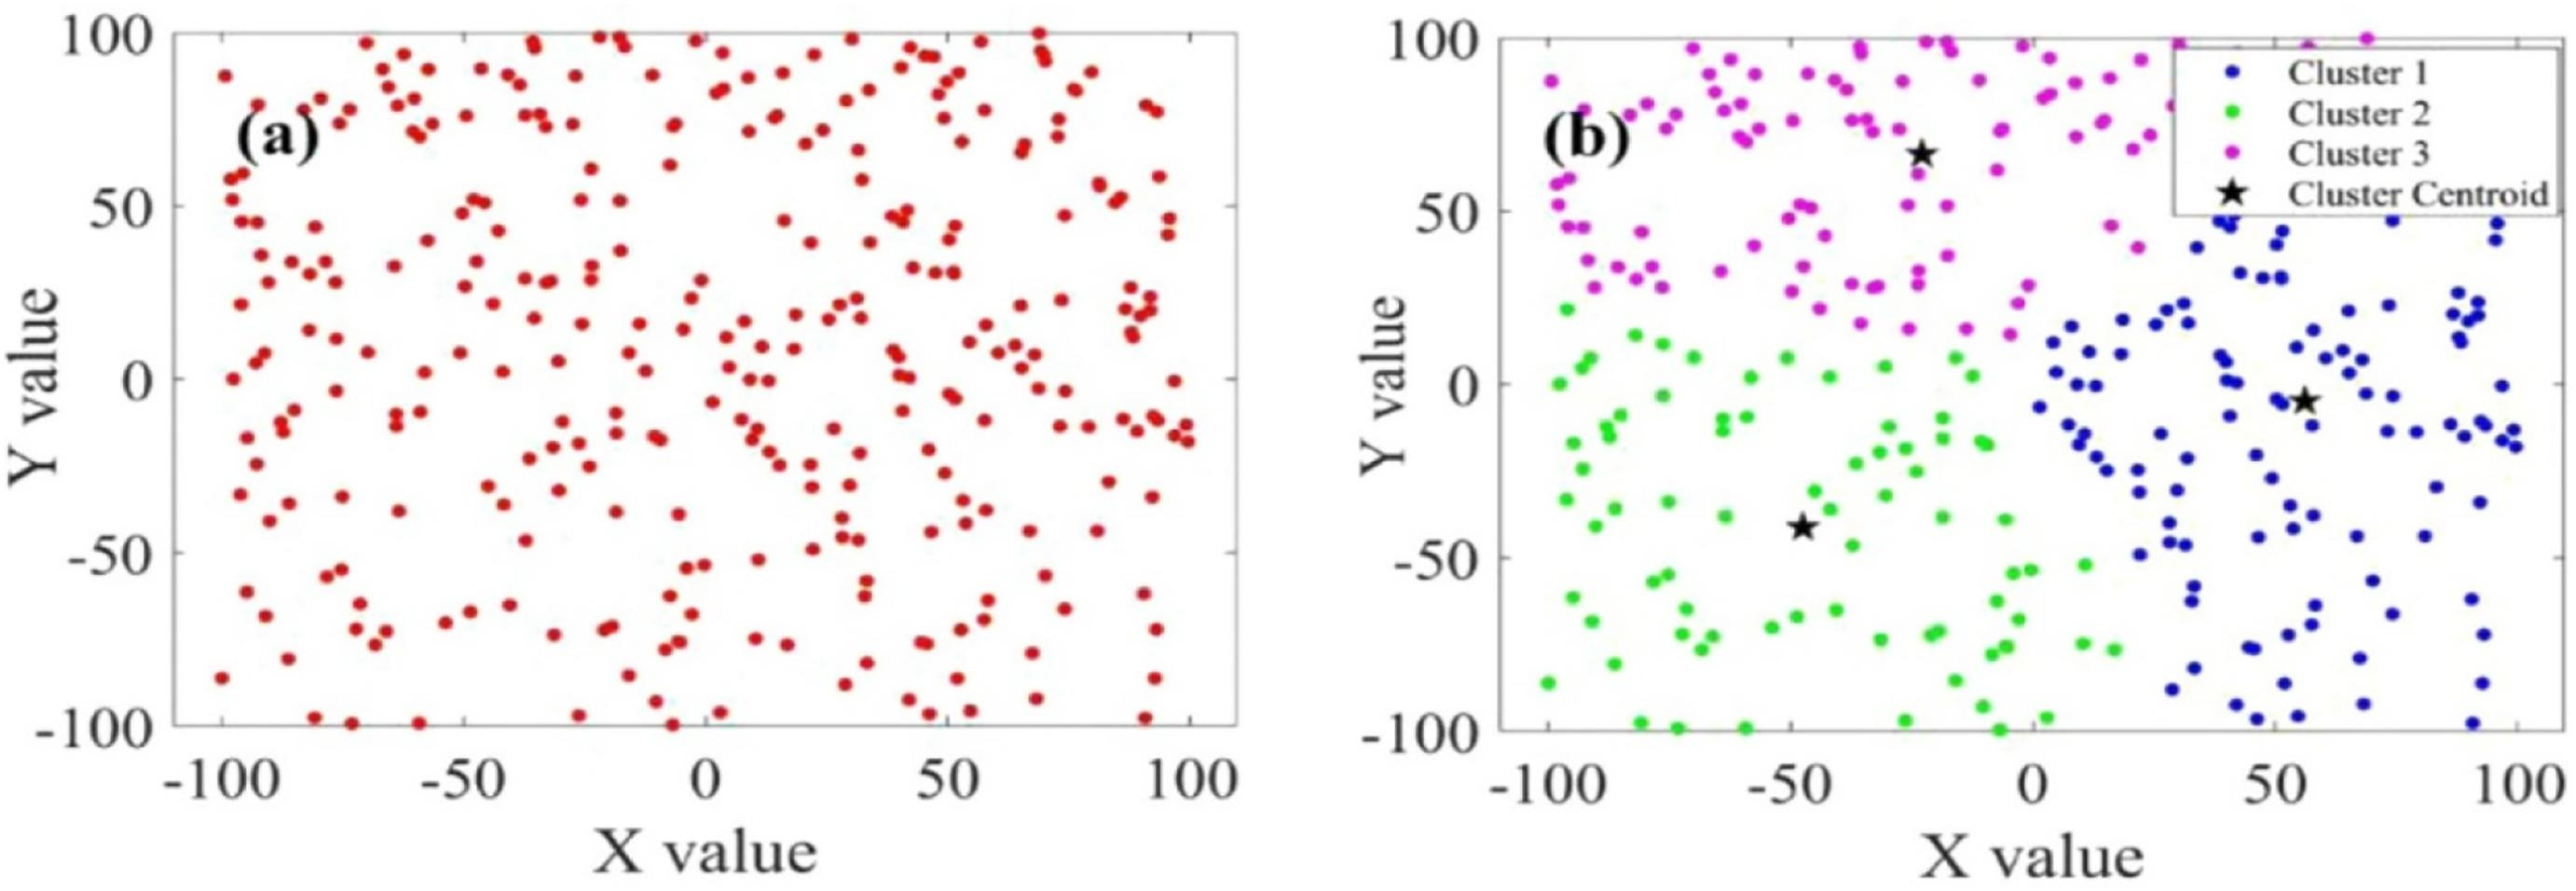
\includegraphics[width=\textwidth]{figures/ref.jpg}
    \caption{K-means clustering: (a) a set of datasets and (b) closest cluster centroid with $K = 3$ \cite{MINH2022109189}}
    \label{brich}
\end{figure}

